\section{Modello di Sviluppo}
\label{modello_di_sviluppo}
Dopo un'attenta lettura del \glo{capitolato} che ha evidenziato la natura a \glo{microservizi} del progetto e dopo una discussione con \Proponente, il gruppo \Gruppo\ ha deciso di adottare, relativamente al ciclo di vita del software, il \textbf{modello incrementale} in modo da garantire la \glo{qualità} e la conformità del prodotto grazie alle maggiori possibilità di poter avere riscontri da parte del proponente. 

\subsection{Modello Incrementale}
\begin{figure}[ht]
    \centering
    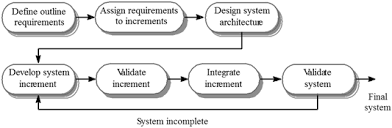
\includegraphics[width=\textwidth]{Immagini/ModelloIncrementale}
    \caption{Modello incrementale, Fonte: \href{https://binaryterms.com/incremental-development-model.html}{binaryterms.com}}
    \label{fig:modello_incrementale}
\end{figure}

In un modello di sviluppo incrementale, sulla base dei requisiti fondamentali e desiderabili trovati durante l'\glo{attività} di analisi, vengono individuati degli incrementi da eseguire. Ogni incremento rappresenta un sottoinsieme delle funzionalità del prodotto finale. I requisiti sono da sviluppare seguendo una priorità (dalla più alta alla più bassa) quindi il rilascio del prodotto non viene mai eseguito in un unico blocco, ma in maniera incrementale.\\
Una volta che gli incrementi sono stati identificati, vengono definiti nel dettaglio i requisiti che devono essere soddisfatti col primo incremento dando il via alla fase di sviluppo dell'incremento stesso. Durante l’attività di sviluppo è lecito aggiungere ulteriori requisiti che devono essere soddisfatti dagli incrementi successivi durante i periodi di \textbf{progettazione di dettaglio, codifica, collaudo} e \textbf{validazione}; non si possono invece andare a modificare i requisiti decisi durante i periodi di \textbf{analisi} e \textbf{progettazione architetturale}. In questo modo al termine di ogni incremento il prodotto software avrà dei miglioramenti o delle funzionalità aggiuntive dalle quali si può ricavare il grado di \glo{efficacia}. Ogni incremento quindi ridurrà il rischio di fallimento e produrrà valore aggiunto.\\
I vantaggi principali del modello di sviluppo incrementale sono:
\begin{itemize}
    \item Ogni incremento permette di avere un riscontro da parte del proponente;
    \item I requisiti a maggior priorità saranno i primi ad essere sviluppati e saranno anche più volte verificati nel corso dello sviluppo;
    \item Al termine di ogni incremento verrà effettuata la verifica dello stesso quindi eventuali errori saranno limitati al singolo incremento;
    \item Dall'incremento corrente è possibile trarre indicazioni su come effettuare il successivo;
    \item Grazie ai rilasci continui è possibile avere anticipatamente un \glo{prototipo} da poter mostrare al proponente.
\end{itemize}

Come richiesto da \Proponente\ la parte di \glo{implementation} riguardante lo sviluppo in figura \S\ref{fig:modello_incrementale} è suddivisa in 4 ulteriori attività:
\begin{itemize}
    \item \glo{\textbf{Sviluppo Locale}};
    \item \glo{\textbf{Testing}};
    \item \glo{\textbf{Staging}};
    \item \glo{\textbf{Produzione}}, equivale all'attività di \glo{deployment} presente in figura \S\ref{fig:modello_incrementale}.
\end{itemize}